\documentclass[11pt,a4]{article}
\usepackage[cm]{fullpage}
\usepackage{graphicx}
\usepackage{subfigure}
\usepackage{epsfig}
\usepackage{epstopdf}
\begin{document}

\begin{figure}[h]
\centering
    \includegraphics[width=0.49\textwidth]{MAX}
    \includegraphics[width=0.49\textwidth]{REST}
    \includegraphics[width=0.49\textwidth]{TBP}
    \includegraphics[width=0.49\textwidth]{SP4}
\caption{Distribution of the distances from all true MPBSs to the center of the closest region predicted by segmentation-based methods for the cell line H1-hESC. All HMM Models were trained with data from H1-hESC and K562 cell lines.}
\label{fig:boxplot.H1hesc.fdr_4.1}
\end{figure}

\begin{figure}[h]
\centering
    \includegraphics[width=0.49\textwidth]{SRF}
    \includegraphics[width=0.49\textwidth]{JUND}
    \includegraphics[width=0.49\textwidth]{GABP}
    \includegraphics[width=0.49\textwidth]{RXRA}
\caption{Distribution of the distances from all true MPBSs to the center of the closest region predicted by segmentation-based methods for the cell line H1-hESC. All HMM Models were trained with data from H1-hESC and K562 cell lines.}
\label{fig:boxplot.H1hesc.fdr_4.2}
\end{figure}

\begin{figure}[h]
\centering
    \includegraphics[width=0.49\textwidth]{USF2}
    \includegraphics[width=0.49\textwidth]{JUN}
    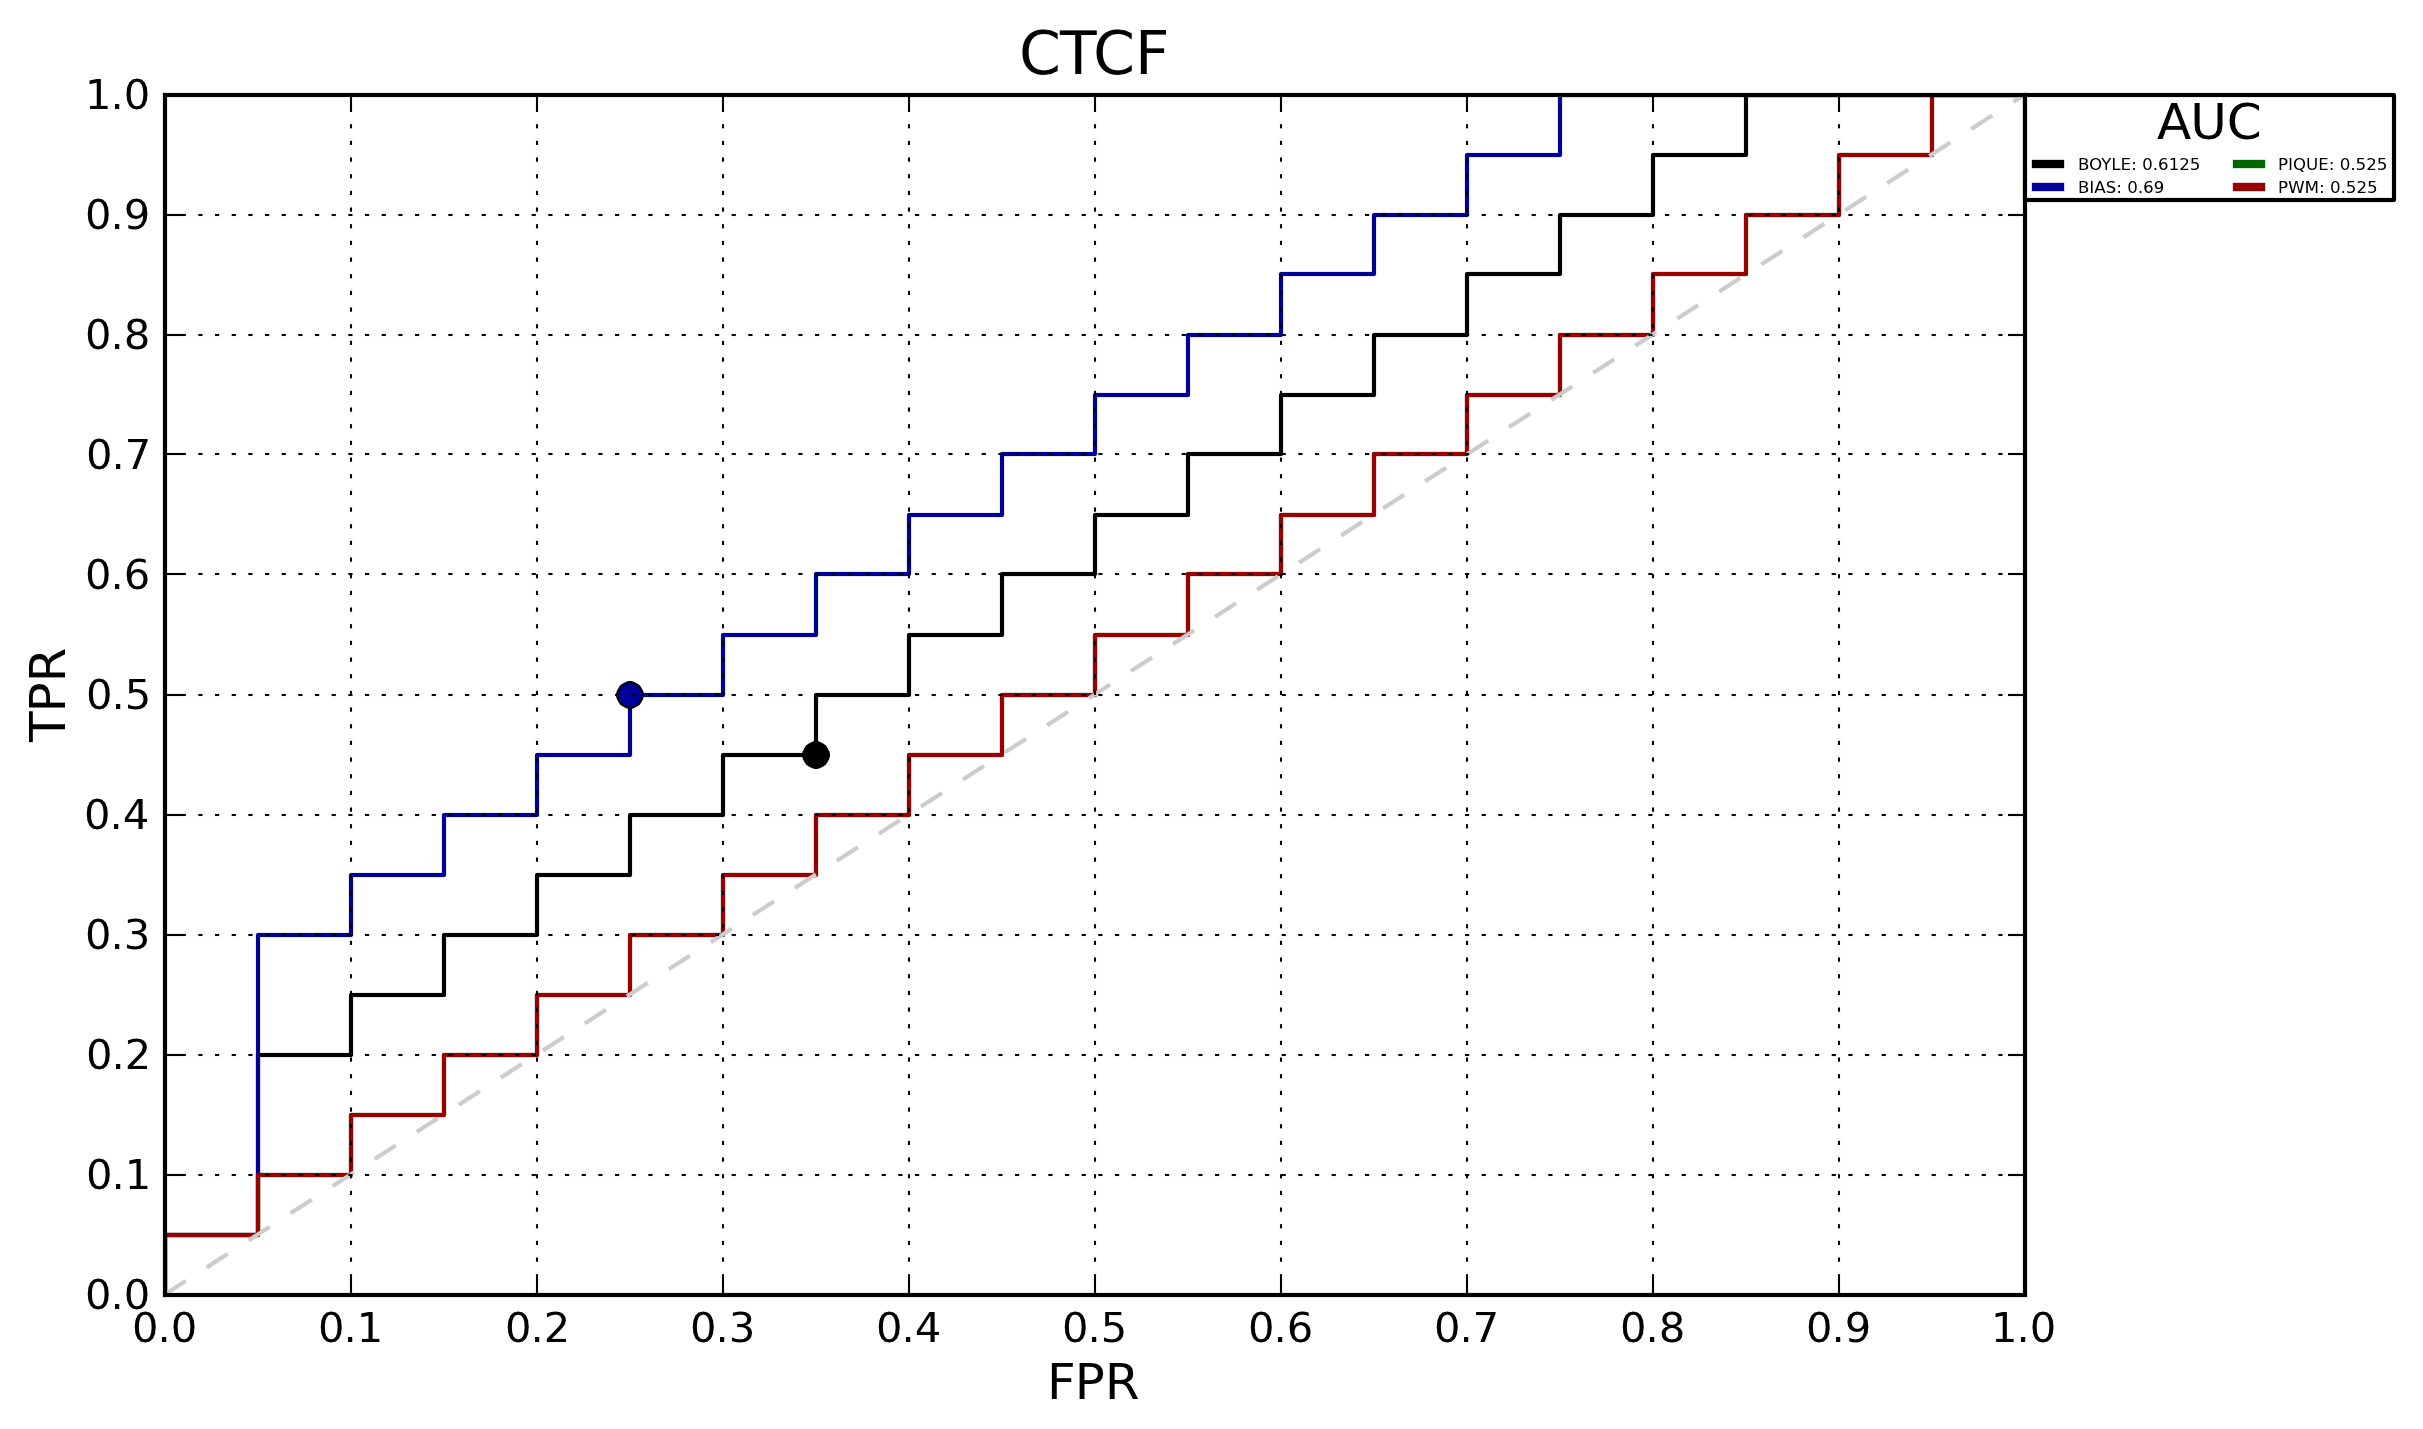
\includegraphics[width=0.49\textwidth]{CTCF}
    \includegraphics[width=0.49\textwidth]{MAFK}
\caption{Distribution of the distances from all true MPBSs to the center of the closest region predicted by segmentation-based methods for the cell line H1-hESC. All HMM Models were trained with data from H1-hESC and K562 cell lines.}
\label{fig:boxplot.H1hesc.fdr_4.3}
\end{figure}

\begin{figure}[h]
\centering
    \includegraphics[width=0.49\textwidth]{BACH1}
    \includegraphics[width=0.49\textwidth]{YY1}
    \includegraphics[width=0.49\textwidth]{FOSL1}
    \includegraphics[width=0.49\textwidth]{SIX5}
\caption{Distribution of the distances from all true MPBSs to the center of the closest region predicted by segmentation-based methods for the cell line H1-hESC. All HMM Models were trained with data from H1-hESC and K562 cell lines.}
\label{fig:boxplot.H1hesc.fdr_4.4}
\end{figure}

\begin{figure}[h]
\centering
    \includegraphics[width=0.49\textwidth]{SP2}
    \includegraphics[width=0.49\textwidth]{TCF12}
    \includegraphics[width=0.49\textwidth]{SP1}
    \includegraphics[width=0.49\textwidth]{MYC}
\caption{Distribution of the distances from all true MPBSs to the center of the closest region predicted by segmentation-based methods for the cell line H1-hESC. All HMM Models were trained with data from H1-hESC and K562 cell lines.}
\label{fig:boxplot.H1hesc.fdr_4.5}
\end{figure}

\begin{figure}[h]
\centering
    \includegraphics[width=0.49\textwidth]{NRF1}
    \includegraphics[width=0.49\textwidth]{RFX5}
    \includegraphics[width=0.49\textwidth]{fdr_4}
    \includegraphics[width=0.49\textwidth]{POU5F1}
\caption{Distribution of the distances from all true MPBSs to the center of the closest region predicted by segmentation-based methods for the cell line H1-hESC. All HMM Models were trained with data from H1-hESC and K562 cell lines.}
\label{fig:boxplot.H1hesc.fdr_4.6}
\end{figure}

\begin{figure}[h]
\centering
    \includegraphics[width=0.49\textwidth]{EGR1}
    \includegraphics[width=0.49\textwidth]{RAD21}
    \includegraphics[width=0.49\textwidth]{ZNF143}
    \includegraphics[width=0.49\textwidth]{P300}
\caption{Distribution of the distances from all true MPBSs to the center of the closest region predicted by segmentation-based methods for the cell line H1-hESC. All HMM Models were trained with data from H1-hESC and K562 cell lines.}
\label{fig:boxplot.H1hesc.fdr_4.7}
\end{figure}

\begin{figure}[h]
\centering
    \includegraphics[width=0.49\textwidth]{CEBPB}
    \includegraphics[width=0.49\textwidth]{USF1}
    \includegraphics[width=0.49\textwidth]{BRCA1}
    \includegraphics[width=0.49\textwidth]{ATF3}
\caption{Distribution of the distances from all true MPBSs to the center of the closest region predicted by segmentation-based methods for the cell line H1-hESC. All HMM Models were trained with data from H1-hESC and K562 cell lines.}
\label{fig:boxplot.H1hesc.fdr_4.8}
\end{figure}

\end{document}